%!TEX root = ..\Master.tex

\section{Dimensionality Reduction}

e.g. finding projection vectors, choosing number of components, applications.\\

motivation:
data compression
speed up learning algorithm


\subsection{PCA}

Principal component analysis is used for reducing the number of dimensions of a feature space.
It works by projecting the data in the feature space, down to a fewer dimensional feature space by minimizing the squared projection error.
The reduced feature space does not nessecarily share the same features, but new features are found which best retains the variance in the data.

PCA should mainly be used for compressing the data to save memory or reducing running time of learning algorithm.
By reducing the amount of features most machine learning algorithms runs faster.
PCA can also be used to prevent overfitting, but its usually better to use regularization. \\

Figure \ref{fig:pca} shows a 3 dimensional feature space where all the data, within a small margin, lies in a 2 dimensional plane.
PCA is used to find two vectors $u^{(1)}$ and $u^{(2)}$ which spans this 2D plane.

\begin{figure}[H]
\centering
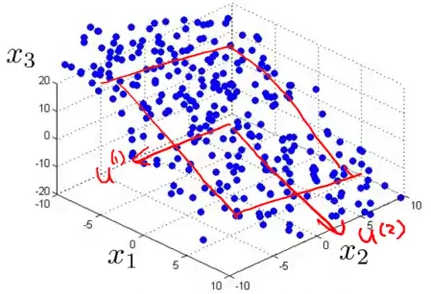
\includegraphics{billeder/pca}
\caption{3D to 2D pca illustration}
\label{fig:pca}
\end{figure}


Preprocessing of the data should be done before doing PCA. \\
Given the training set:
\begin{equation}
x = 
\begin{bmatrix}
x_1 & x_2 & \dots & x_m
\end{bmatrix}
\end{equation}

Ensure that every feature has zero mean by doing mean normalization:
\begin{equation}
\mu_j = \frac{1}{m} \sum^m_{i=1} x_j^{(i)}
\end{equation}
\begin{equation}
x_j = x_j - \mu_j
\end{equation}

Feature scaling can also be done if the features have very different value ranges. TODO \\

After preprocessing the data, we can do PCA on it.\\
We start by computing the covariance matrix $\Sigma$:
\begin{equation}
\Sigma = \frac{1}{m} \sum^n_{i=1} x^{(i)} {x^{(i)}}^T
\end{equation}

The covariance matrix descripes how the different features relates.
When doing feature reduction we want to remove features which has high correlation with other features.
An example could be a feature which descripes a length in cm and another feature descriping the same length in inches.
These features will have very high correlation and one of them can be removed from the feature space without loosing much information. \\

Then we compute the eigenvectors of covariance matrix:
\begin{equation}
U = \begin{bmatrix}
   u^{(1)} & u^{(2)} & \dots & u^{(n)}
 \end{bmatrix}
\in \mathbb{R}^{n \times n}
\end{equation}

The eigenvectors will lay in the directions of most variance in the data.
This is what is shown on Figure \ref{fig:pca}.
The longer the eigenvector, the more variance it descripes.
Therefore we want to keep the longest eigenvectors and remove the shortest eigenvectors.

The eigenvectors are ordered by length in the matrix $U$.
The longest is the first. \\

We select the first $k$ eigenvectors to get the reduced set of eigenvectors:
\begin{equation}
U_{reduce} = \begin{bmatrix}
   u^{(1)} & u^{(2)} & \dots & u^{(k)}
 \end{bmatrix}
\end{equation}

We can now calculate the new feature vectors:
\begin{equation}
z = U_{reduce}^Tx
\end{equation}

We have now reduced the feature space to a $k$ dimensional feature space.
Say we want to retain at least $95\%$ of the variance in the data.
We do this by picking the smallest value of $k$ so that:
\begin{equation}
\frac{\displaystyle\sum^{k}_{i=1} S_{ii}}{\displaystyle\sum^{n}_{i=1} S_{ii}} \geq 0.95
\end{equation}

The matrix $S$ is found by doing singular value decomposition (SVD). The matrix $S$ has the form:
\begin{equation}
S =  
\begin{bmatrix}
S_{11} & 0 & 0 & 0 & 0 \\
0 & S_{22} & 0 & 0 & 0 \\
0 & 0 & S_{33} & 0 & 0 \\
0 & 0 & 0 & \dots & 0 \\
0 & 0 & 0 & 0 & S_{nn} \\
\end{bmatrix}
\end{equation}

In our project we use PCA to reduce our feature space from 64 dimensions down to 40 dimensions.
We do this to increase the speed of our learning algorithms while still retainging almost all of our data ($\geq 99.99\%$) as seen on Figure \ref{fig:pca-on-our-data}.
(TODO: Add axis labels to figure. x = number of features. y = retained variance.)

\begin{figure}[H]
\centering
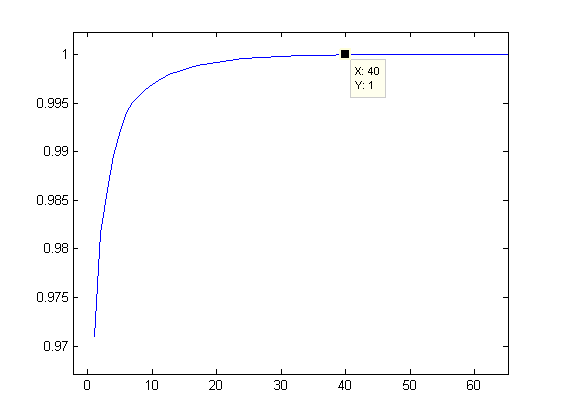
\includegraphics{billeder/pca-on-our-data}
\caption{3D to 2D pca illustration}
\label{fig:pca-on-our-data}
\end{figure}

\subsection{Fisher}

Introtext\\

Math\\

How we use it or why we don't use it\\

Intermediate result\\

%------------------------------------------------